\section{Groups: a brief introduction}\label{sec:Groups}
\textit{The formulas in this section are from book \cite{Quark_Lepton}.}

Group theory is a branch of mathematics that underlines the treatment of symmetry. It plays an very important role particle physics. Some basic concepts and terminologies for the group theory will be given in this section. Here we use operators of 3D rotation ($R(\theta_1,\theta_2,\theta_3)$), the $\theta_i$ means the rotated angle respect to each axis) as an example. Suppose all the rotation form a rotation group and the ``multiplication'' of two rotations $R_2 R_1$ means first do rotation $R_1$ then do $R_2$, then this group must full fill following four requirements: 1, the $R_2 R_1$ should equal to an other group element $R_3$. This is correct for the rotation because two rotations can be expressed by one rotation; 2, the existence of identity element. This is satisfied by the existence of a rotation $R(0,0,0)$; 3, the existence of an inverse element for each element. This is satisfied by the existence of $R(-\theta_1,-\theta_2,-\theta_3)$ with respect to $R(\theta_1,\theta_2,\theta_3)$; 4, the equality of $(R_1 R_2) R_3$ and $R_1 (R_2 R_3)$. This is also correct obviously. It should be noticed that it is not necessary to have $R_1 R_2=R_2 R_1$ for a group.

As we know the experiment result or the physics is not dependent with the orientation of the laboratory. Therefore the rotation group is a symmetry group. Suppose the transformation of system state by the rotation $R$ is
$$|\psi\rangle\rightarrow|\psi^{'}\rangle=U|\psi\rangle$$

and the probability of a system described by $|\psi\rangle$ will be found in state $|\varphi\rangle$ must unchanged by $R$,
$$|\langle\varphi|\psi\rangle|^{2}=|\langle\varphi^{'}|\psi^{'}\rangle|^{2}=|\langle\varphi| U^{\dag}U|\psi\rangle|^{2}.$$
So the $U^{\dag}U=1$ and $U$ is unitary operator. Besides, the rotation $R$ can be represented by $U$. Because the rotation group is Lie group which has a crucial property that is each rotation can by expressed by a product of succession of infinitesimal rotations. For instance, the rotation on z axis with infinitesimal angle $\epsilon$, to first order $\epsilon$, can by expressed by 
$$U=1-i\epsilon J_z$$
where the $J_z$ is called the generator of the rotations about the z axis. Now 
$$1=U^{\dag}U=(1+i\epsilon J_z^{\dag})(1-i\epsilon J_z)\\=1+ i\epsilon(J_z^{\dag}-J_z)+0(\epsilon^{2}),$$
it gives $J_z^{\dag}=J_z$ which means $J_z$ is hermitian and hence is a observable.

\subsection{SU(2) groups}\label{subsec:SU2_groups}

In the lowest-dimension nontrivial representation of the rotation group, the generators can be written as
$$J_i=\frac{1}{2}\sigma_i,~\mathrm{with}~i=1,2,3,$$
where the $\sigma_i$ is Pauli matrices
\begin{equation}
\begin{split}
&\sigma_1=\begin{pmatrix} 0 & 1 \\ 1 & 0 \end{pmatrix},~\sigma_2=\begin{pmatrix} 0 & -i \\ i & 0 \end{pmatrix},~\sigma_3=\begin{pmatrix} 1 & 0 \\ 0 & -1 \end{pmatrix}
\end{split}
\label{eq:pauli_matrix}
\end{equation}
and the base states for this representation is conventionally chosen to be the eigenvectors of $\sigma_3$, that is 
\begin{equation}
\begin{split}
\begin{pmatrix}  1 \\  0 \end{pmatrix}~~\mathrm{and}~~\begin{pmatrix}  0 \\  1 \end{pmatrix}
\end{split}
\label{eq:base_state}
\end{equation}
which describes spin $\frac{1}{2}$ particle with spin up spin and spin down in z direction or it can describe the isospin state of proton ($+\frac{1}{2}$) and neutron ($-\frac{1}{2}$) because they are indistinguishable in nuclear interaction.
The unitary transformation matrices can by written as
$$U(\theta_i)=e^{-i\theta_i \sigma_i/2}.$$
The set of all 2$\times$2 unitary matrices is known as the group $U(2)$. However, the $U(2)$ is larger then the $U(\theta_i)$, because all elements in $U(\theta_i)$ has zero trace. For any zero trace hermitian matrix $\sigma$, it can be proved that 
$$\mathrm{det}(\sigma)=e^{iTr(\sigma)}=1.$$
Therefore, all traceless 2$\times$2 unitary matrices $U(\theta_i)$ form a subgroup of $U(2)$, which is call $SU(2)$ group, the ``S'' means special. 

\subsection{SU(3) groups}\label{subsec:SU3_groups}
All 3$\times$3 unitary matrices with det$U=1$ form a $SU(3)$ group. There are $3^{2}-1=8$ linearly independent hermitian generators.

The fundamental representation of $SU(3)$ group is a triplet. The three colors (R, G, B) of a quark form a fundamental representation of a $SU(3)$ group. In this representation, the 8 generators are 3$\times$3 traceless unitary matrices and are traditionally called $\lambda_i$ with $i$ from 1 to 8. There are only two diagonal generator matrices which are

\begin{equation}
\begin{split}
&\lambda_3=\begin{pmatrix}  1&0&0\\0&-1&0\\0&0&0 \end{pmatrix}~~\mathrm{and}~~\lambda_8=\sqrt{\frac{1}{3}}\begin{pmatrix}  1&0&0\\0&1&0\\0&-2&0 \end{pmatrix}
\end{split}
\label{eq:lam3_8}
\end{equation}
with simultaneous eigenvectors  
\begin{equation}
\begin{split}
&R=\begin{pmatrix}  1\\0\\0\end{pmatrix},~~G=\begin{pmatrix}  0\\1\\0\end{pmatrix},~~B=\begin{pmatrix}  0\\0\\1\end{pmatrix}
\end{split}
\label{eq:RGB}
\end{equation}
These states are plotted in Figure \ref{fig:SU3} in term of their $\lambda_3$ and $\lambda_8$ eigenvalues. The figure also shows how the base states are transformed using the $\lambda_i$ generators. The $\lambda_i$ are known as the Gell-Mann matrices (see \ref{subsec:Feynman_QCD}), the $\lambda_1$, $\lambda_2$, and $\lambda_3$ correspond to the three Pauli matrices, which means they exhibit explicitly one $SU(2)$ subgroup of $SU(3)$.

\begin{figure}[h!]
 \begin{center}
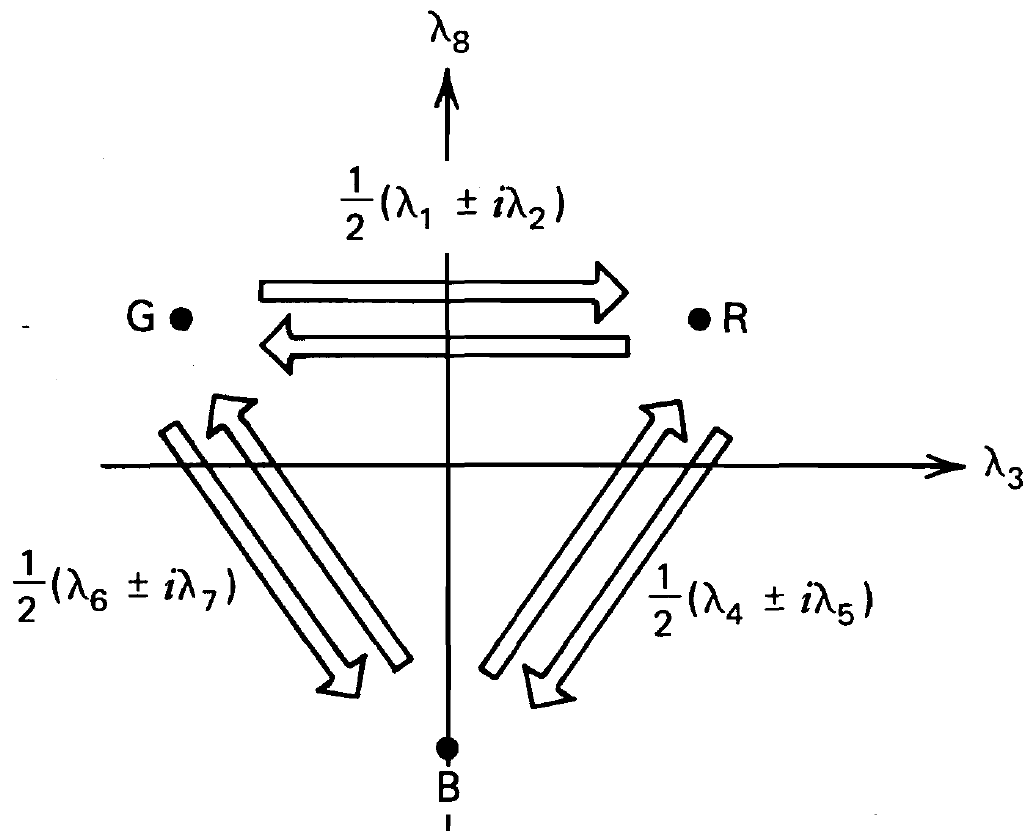
\includegraphics[width=0.5\textwidth]{figures/theory/SU3.png}
\caption{The action of the generators on fundamental representations of $SU(3)$ \cite{Quark_Lepton}.}
  \label{fig:SU3}
 \end{center}
\end{figure}
